 \documentclass[a4paper,12pt]{article}
\usepackage[a4paper,top=1.3cm,bottom=2cm,left=1.5cm,right=1.5cm,marginparwidth=0.75cm]{geometry}
\usepackage{setspace}
\usepackage{cmap}					
\usepackage{mathtext} 				
\usepackage[T2A]{fontenc}			
\usepackage[utf8]{inputenc}			
\usepackage[english,russian]{babel}
\usepackage{multirow}
\usepackage{graphicx}
\usepackage{wrapfig}
\usepackage{tabularx}
\usepackage{float}
\usepackage{longtable}
\usepackage{hyperref}
\hypersetup{colorlinks=true,urlcolor=blue}
\usepackage[rgb]{xcolor}
\usepackage{amsmath,amsfonts,amssymb,amsthm,mathtools} 
\usepackage{icomma} 
\mathtoolsset{showonlyrefs=true}
\usepackage{euscript}
\usepackage{mathrsfs}

\DeclareMathOperator{\sgn}{\mathop{sgn}}
\newcommand*{\hm}[1]{#1\nobreak\discretionary{}
	{\hbox{$\mathsurround=0pt #1$}}{}}


\title{\textbf{Изучение колебаний струны (1.4.5)}}
\author{Павлушкин Вячеслав}
\date{November 2021}


\begin{document}
	
	\maketitle
	
	\section{Введение}
	
	\textbf{Цели работы:} изучение поперечных стоячих волн на струне; определение собственных частот колебаний струны; исследование зависимости скорости распространения поперечных волн на струне в зависимости от её натяжения.\\
	\textbf{Оборудование:} закрепленная на станине стальная струна, набор грузов,
	электромагнитные датчики, звуковой генератор, двухканальный осциллограф, частотомер.
	
	\section{Теоретические сведения}
	
	Основное свойство струны -- гибкость, является следствием ее большой длины по сравнению с поперечными размерами. Даже струны, изготовленные из жестких материалов, практически не сопротивляются изгибанию, если размер изгибаемого участка значительно больше поперечного размера струны. Данный факт позволяет не учитывать при дальнейшей работе изгибные напряжения.
	
	Горизонтально закрепленная струна провисает под действием поля тяжести, при отсутствии натяжения. Достаточно натянутую струну можно считать прямой, если ее концы закреплены на одном горизонтальном уровне. Учитывая этот факт, в дальнейшем действие силы тяжести учитываться не будет.
	
	Натянутая струна с жестко закрепленными концами удобна для изучения колебаний. Это связанно с тем, что в струне можно непосредственно наблюдать простейшие типы колебаний и волн, измерять их параметры и сравнивать результаты наблюдения с результатами теоретических расчетов.
	
	Движение элементов струны может быть вызвано изменением ее формы или передачей ей импульса. Натяжение струны стремиться вернуть ее в изначальное прямолинейное положение, и это приводит к тому, что возникает движение элементов струны. Возмущения бегут вдоль струны.
	
	Скорость распространения подобного возмущения можно вычислить по формуле \eqref{velocity_of_deformation}.
	
	\begin{equation}
		u = \sqrt{\frac{T}{\rho_l}}
		\label{velocity_of_deformation}
	\end{equation}
	где $F$ -- сила натяжения струны, $\rho_{l}$ -- масса струны на единицу длины.
	
	При заданной частоте $\nu$ длина волны определяется по формуле:
	
	\begin{equation}
		\lambda = \frac{u}{\nu}
	\end{equation}
	
	Частоты собственных колебаний струны определяются формулой:
	
	\begin{equation}
		\nu_{n} = \frac{nu}{2l} = \frac{n}{2l}\sqrt{\frac{T}{\rho_l}}
		\label{frequency_velocity_equation}
	\end{equation}
	где $n$ -- число полуволн, $l$ -- длина струны.
	
	\section{Экспериментальная установка}
	
	\begin{figure}[h!]
		\begin{center}
			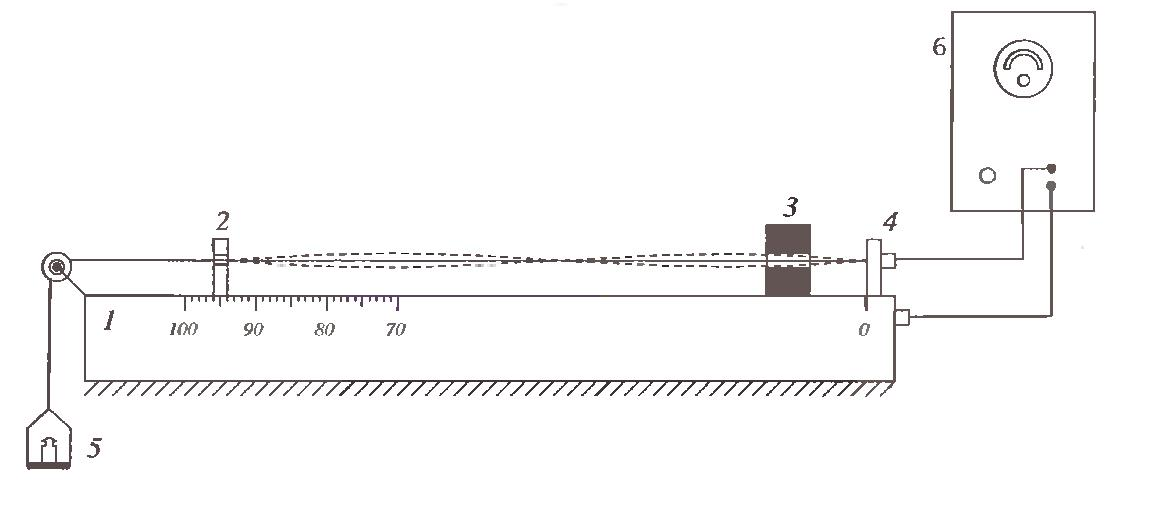
\includegraphics[width = 0.9\textwidth]{1.4.5 ustan}
			\caption{Схема экспериментальной установки}
			\label{facility}
		\end{center}
	\end{figure}
	
	На Рисунке \ref{facility} представлена схема экспериментальной установки. Устроена она следующим образом: на массивной металлической рейке 1 установлены опора 2 и магнит 3, которые можно перемещать вдоль рейки, а также неподвижная опора 4. Один конец струны закреплен в изоляторе опоры 4. От него струна проходит между полюсами магнита и через опору 2, которая дает возможность струне перемещаться в горизонтальной плоскости, неподвижный блок и соединяется с чашкой 5, на которую помещаются грузы. Такое устройство позволяет регулировать натяжение струны.  К концу струны, закрепленному в изоляторе опоры 4, и к массивной металлической рейке 1 подводится переменное напряжение от звукового генератора 6. Движение струны вызывается силой Ампера, действующей на проводник с током со стороны магнитного поля. Частота колебания струны совпадает с частотой вынуждающей силы, т.е с частотой силы Ампера. Так как данная сила зависит от тока в проводнике, то частота колебаний струны будет совпадать с частотой генератора.
	
	В натянутой струне возникнуть колебания, которые сложившись после отражения от опор 2 и 4 создадут стоячую волну, если на длине струны уложится целое число полуволн.
	
	\section{Задание}
	\subsection{Визуальное наблюдение стоячих волн}
	
	Для натяжения струны подвесим 2 грузика массами $500,9 \text{, г}$ и $482\text{, г}$, тогда сила натяжения: $T_1 = (M_1 + M_2 + M_\text{плат})g = (0,5009 + 0,482 + 0,1193)9,81  = 10,813 \text{, Н}$. По формуле \eqref{frequency_velocity_equation}, где масса струны на единицу длины $\rho_l = 568,4\text{, мг}/\text{м}$, получаем, что: $\nu_1^{\text{выч}} = 137,9\text{, Гц}$.
	
	Посредством возбуждения стоячей волны на основной гармонике находим частоты визуально наблюдаемых гармоник:
	\begin{table}[!h]
		\begin{center}
			\begin{tabular}{|c|c|c|c|c|}
				\hline
				$\nu_1$, Гц &$\nu_2$, Гц& $\nu_3$, Гц& $\nu_4$, Гц& $\nu_5$, Гц\\
				\hline
				140,1 & 280,3 & 412,7 & 560,4& 692,5\\
				\hline 
			\end{tabular}
		\caption{Частоты наблюдаемых гармоник}
		\end{center}
	\end{table}

	\subsection{Регистрация стоящих волн с помощью осциллографа}
	
	С помощью осциллографа будем находить частоты гармоник с 1 до 11. Изменяя массы грузов получаем таблицу:
	\begin{table}[!h]
		\begin{center}
			\begin{tabular}{|c|c|c|c|c|c|c|c|c|c|c|c|}
				\hline
				$T$, Н& $\nu_1$, Гц &$\nu_2$, Гц& $\nu_3$, Гц& $\nu_4$, Гц& $\nu_5$, Гц& $\nu_6$, Гц &$\nu_7$, Гц& $\nu_8$, Гц& $\nu_9$, Гц& $\nu_{10}$, Гц & $\nu_{11}$, Гц\\
				\hline
				10,8 & 139,9 & 276,8 & 415,7 & 554,6 & 693,5 & 833,5 & 978,3 & 1121,2 & 1253,1 & 1380,1 & 1536,9 \\ 
				\hline
				14,1 & 156,7 & 318,4 & 482,1 & 629,8 & 801,5 & 948,2 & 1136,9 & 1268,6 & 1430,2 & 1593,1 & 1734,7 \\ 
				\hline
				18,6 & 179,7 & 359,3 & 543,1 & 731,8 & 898,5 & 1092,2 & 1273,9 & 1460,6 & 1617,3 & 1802,1 & 1983,7 \\
				\hline
				22,8 & 194,5 & 393,2 & 602,5 & 804,1 & 1020,1 & 1213,2 & 1413,5 & 1600,1 & 1802,2 & 1996,9 & 2225,5 \\ 
				\hline
				27,4 & 215,4 & 431,8 & 649,2 & 880,6 & 1097,1 & 1326,4 & 1561,1 & 1765,2 & 1974,6 & 2194,3 & 2413,4 \\ 
				\hline
			\end{tabular}
		\caption{Снятые результаты частот гармоник}
		\end{center}
	\end{table}

	Построим график зависимости $\nu_n$ от $n$ по МНК:
	
	\begin{figure}[h!]
		\begin{center}
			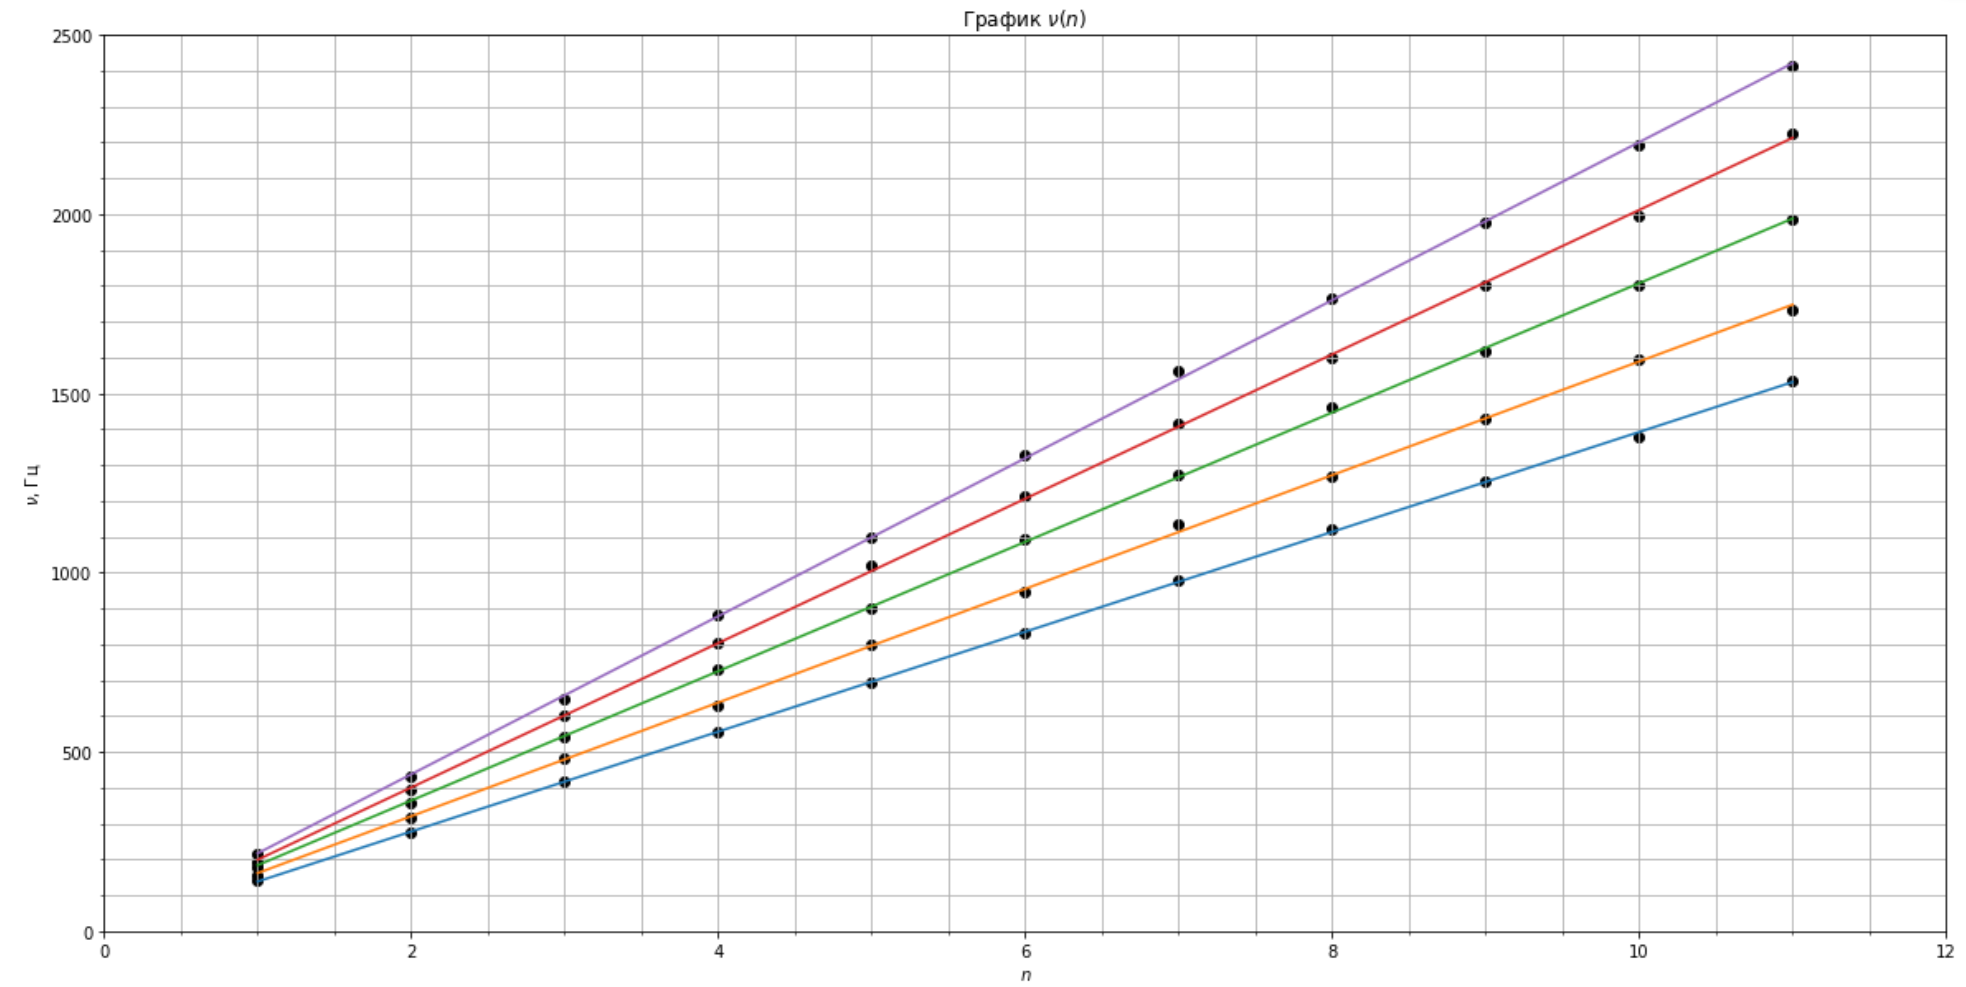
\includegraphics[width = 0.9\textwidth]{1.4.5 graph}
			\caption{График зависимости $\nu_n (n)$}
		\end{center}
	\end{figure}
	
	Воспользуемся формулой \eqref{frequency_velocity_equation}, получаем, что угол наклона графика $k = \dfrac{u}{2l}$. По формулам МНК найдем коэффиценты наклона для каждой прямой и их случайные погрешности:
	
	\begin{equation}
		k=\frac{\langle n\nu\rangle-\langle n\rangle \langle \nu\rangle}{\langle n^2\rangle - \langle n\rangle^2},
	\end{equation}

	\begin{equation}
		\sigma_k^\text{случ}=\frac{1}{\sqrt{N}}\sqrt{\frac{\langle \nu^2 \rangle - \langle \nu \rangle^2}{\langle n^2 \rangle - \langle n \rangle^2} - k^2  },
	\end{equation}
	
	\begin{equation}
		\sigma_k^{\text{сист}} = \sqrt{ \varepsilon_\nu^2 + \varepsilon_l^2 }
	\end{equation}

	\begin{equation}
		\sigma_k = \sqrt{\sigma_\text{случ}^2 + \sigma_\text{сист}^2}
	\end{equation}

	Посчитав все погрешности, коэффиценты наклона и из них найдем $u$, получаем таблицу:
	
	\begin{table}[H]
		\begin{center}
			\begin{tabular}{|c|c|c|c|c|c|}
				\hline
				$T\text{, Н}$ & 10,8&14,1& 18,6&22,8&27,4\\
				\hline
				$u\text{, м/с}$  & 139,3 & 158,6 & 180,4 & 201,4 & 220,4 \\ \hline
				$\sigma_{u}^{\text{случ}} \text{, м/с}$     & 0,5   & 1   & 0,8   & 1   & 0,9    \\ \hline
				$\sigma_{u}^{\text{сист}} \text{, м/с}$ & 1,4  & 1,6 & 1,8   & 2   & 2,2     \\ \hline
				$\sigma_{u} \text{, м/с}$ & 1,5   & 1,9   & 2   & 2,2   & 2,4    \\ \hline
			\end{tabular}
		\caption{Полученные скорости с погрешностями}
		\end{center}
	\end{table}

	Средняя относительная погрешность измерения скорости распространения колебаний $\varepsilon_u \approx 1,1\% $. Полученные значения скорости:
	
	\begin{itemize}
		\item $T = 10,8$, Н -- $u = (139,3 \pm 1,5)$, м/с
		\item  $T = 14,1$, Н -- $u = (158,6 \pm 1,9)$, м/с
		\item  $T = 18,6$, Н -- $u = (180,4 \pm 2)$, м/с
		\item  $T = 22,8$, Н -- $u = (201,4 \pm 2,2)$, м/с
		\item  $T = 27,4$, Н -- $u = (220,4 \pm 2,4)$, м/с
	\end{itemize}

	С помощью полученных данных построим график зависимости $u^2(T)$, для того, чтобы найти погонную плотность струны $ \rho_l $. 
	
	\begin{figure}[h!]
		\begin{center}
			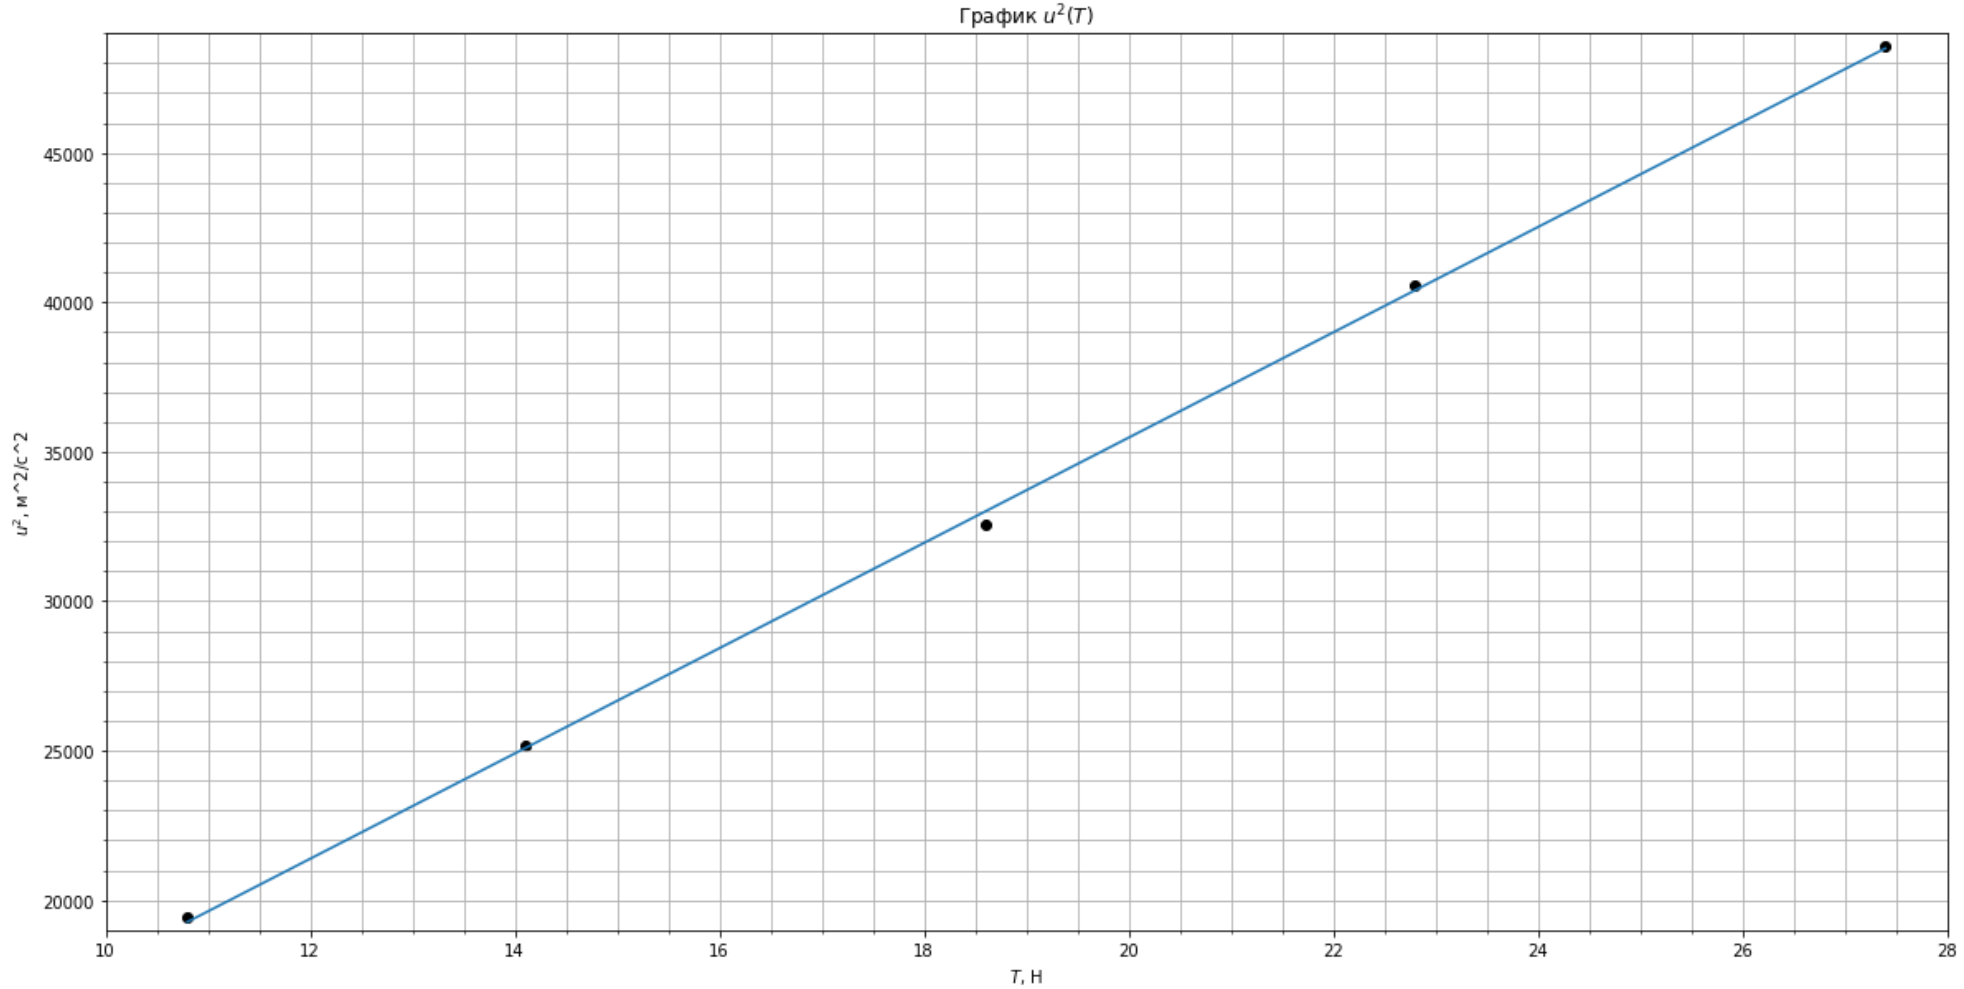
\includegraphics[scale=0.53]{1.4.5 grapg2}
			\caption{Зависимость $ u^2 $ от $ T $}
			\label{1.4.5 grapg2}
		\end{center}
	\end{figure}

	С помощью формулы \eqref{velocity_of_deformation}, можно понять, что коэффицент наклона $k$, для графика \ref{1.4.5 grapg2}, будет равен: $$k = \dfrac{1}{\rho_l}$$. График был построен по МНК, а значит $k$ и его погрешность можно найти по формулам:
	
	\begin{equation}
		k=\frac{\langle Tu^2\rangle-\langle T\rangle \langle u^2\rangle}{\langle T^2\rangle - \langle T\rangle^2} \approx 1760,7 \text{, $\dfrac{\text{м}}{\text{кг}}$},
	\end{equation}
	
	\begin{equation}
		\sigma_k^\text{случ}=\frac{1}{\sqrt{N}}\sqrt{\frac{\langle u^4 \rangle - \langle u^2 \rangle^2}{\langle T^2 \rangle - \langle T \rangle^2} - k^2  } \approx 22,5\text{, $\dfrac{\text{м}}{\text{кг}}$},
	\end{equation}
	
	\begin{equation}
		\sigma_k^{\text{сист}} = \sqrt{ \varepsilon_{u^2}^2 + \varepsilon_T^2 } \approx 38,7\text{, $\dfrac{\text{м}}{\text{кг}}$},
	\end{equation}
	
	\begin{equation}
		\sigma_k = \sqrt{\sigma_\text{случ}^2 + \sigma_\text{сист}^2} \approx 44,8\text{, $\dfrac{\text{м}}{\text{кг}}$},
	\end{equation}

	Таким образом $k = (1760,7 \pm 44,8) {, \dfrac{\text{м}}{\text{кг}}} $.
	Тогда \underline{ $\rho_l = (576,9 \pm 14,4) \text{, $\dfrac{\text{мг}}{\text{м}}$}$}.
	
	Полученное значение соответствует истинному значению погонной плостности струны, которая равняется $\rho^{\text{ист}}_l = 568,4\text{, $\dfrac{\text{мг}}{\text{м}}$} $. 
	\section{Вывод}
	
	\begin{enumerate}
		\item Во время выполнения работы было подтверждено несколько теоретических зависимостей между физическими величинами. С точностью $\varepsilon_{\nu_{1}} = 0,01$ подтверждена формула для определения частот гармоники струны. С точностью  $\varepsilon_{u} = 0,011$ подтверждена формула для определения скорости распространения волны в твердом теле под действием внешней силы.
		\item Полученные графики имеют вид, предсказанный теоретически. Относительно большое значение относительной погрешности определения частоты 11 гармоники для массы нагрузки, соответствующей 3 грузам, объясняется ошибочным измерением частоты данной гармоники, что видно из графика. 
		\item С точностью $ \varepsilon_{\rho_{l}} = 0,026 \%$ определена линейная плотность струны, значение которой совпало со значением, указанным на данной установке.
	\end{enumerate}
\end{document}
